\section{Implementing a web application for DOT}
In this section, we'll implement a browser base 
application by using \textbf{Dash}. Dash is a 
Python framework for building web applications. 
It built on top of Flask, Plotly. js, React, and 
React Js. It enables you to build dashboards using 
pure Python. Dash is open-source, and its apps run 
on the web browser.
In this section, we don't dig into the details of 
the codes. The steps are similar to the previous 
section. The application UI has Three parts:
\begin{enumerate}
    \item Text Area for wrting the code
    \item A section for printing Errors
    \item A section for showing the graph
\end{enumerate}

\begin{figure}[H]
\centering
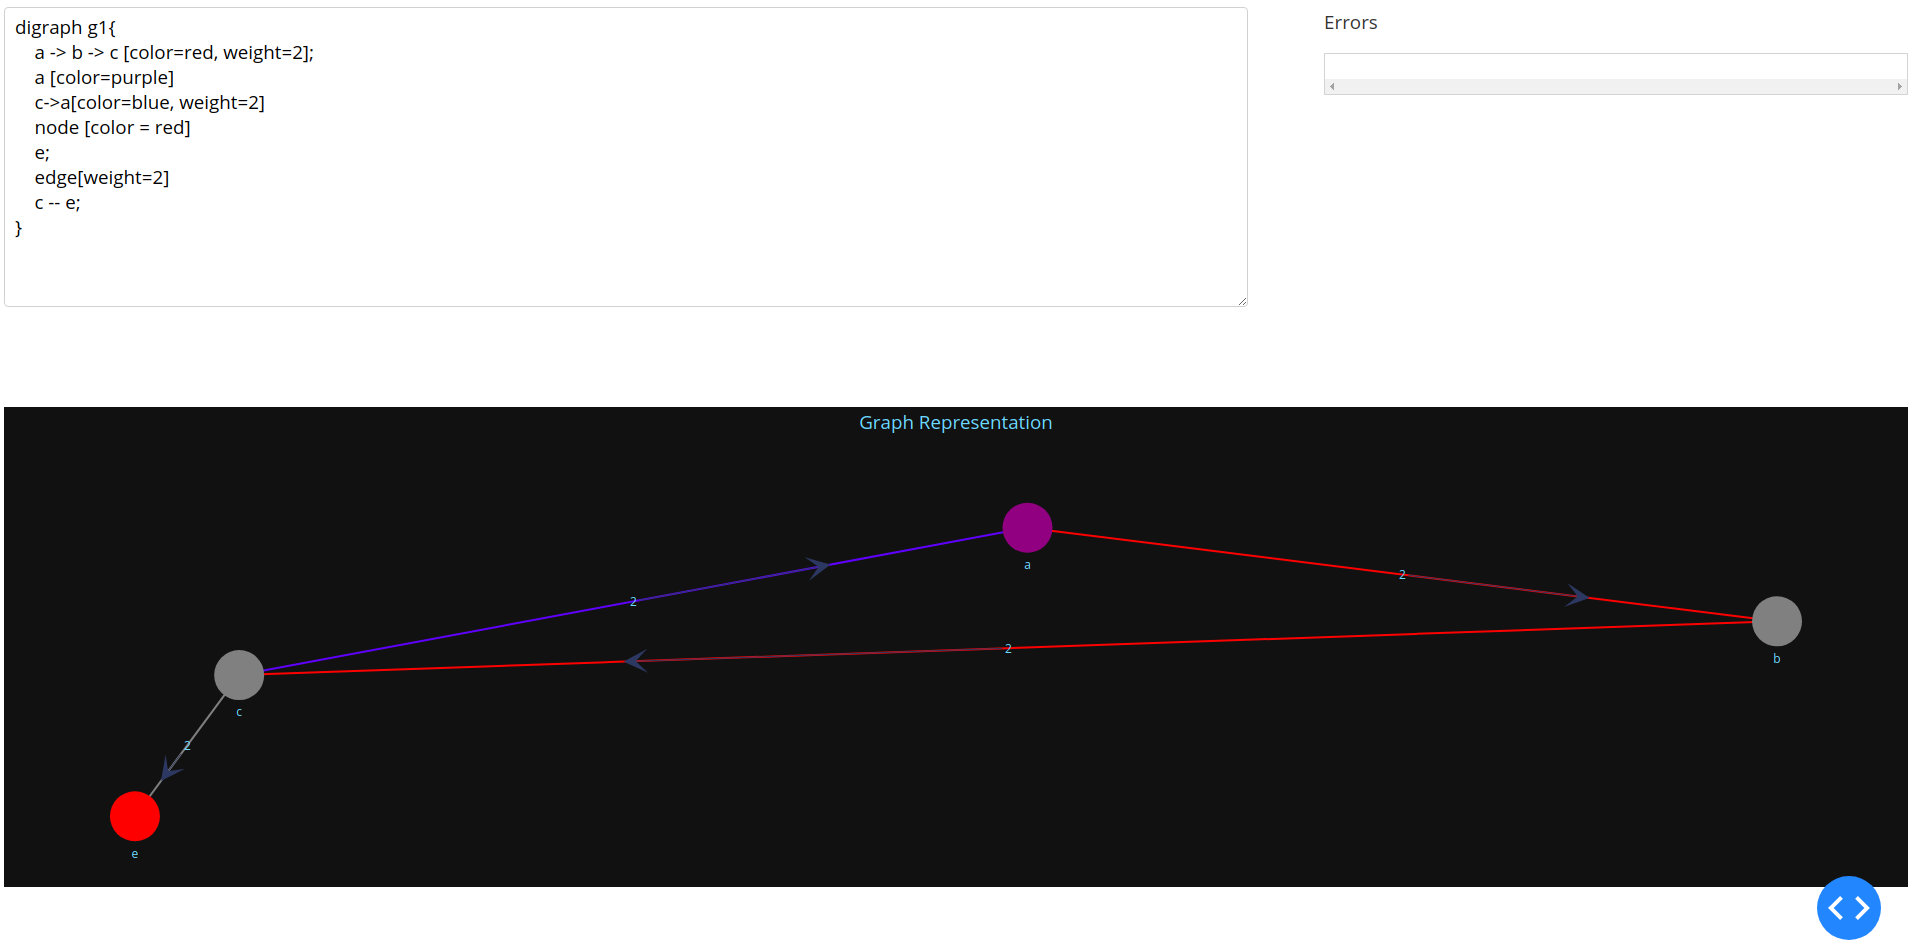
\includegraphics[width=\linewidth]{images/dash-app.png}
\caption{Dash application for DOT}
\end{figure}
To show the errors a custom ErrorListener is written in python. The code is shown
in the Listing \ref{list:ErrorListener}
\pythonexternal[caption=Custom listener written in python,label=list:ErrorListener]{../src/main-generated/DOTErrorListener.py}
For seeing whole codes visit github repository:
\newline
\par \href{https://github.com/m3hransh/DOT_Lang}{https://github.com/m3hransh/DOT\_Lang}